\chapter{A combustão: do que o fogo precisa}\label{ch:g4:what-a-fire-needs}

Uma fogueira ao entardecer. Ela precisou de lenha seca, de um fósforo
para começar, e o vento que passa por ela a mantém viva. Depois de uma
hora, as toras encolheram até virar brasas incandescentes e cinza
branca, e uma fumaça cinzenta foi embora para o céu. Para onde foi a
madeira? Do que um fogo precisa, e o que ele deixa para trás?

\begin{recall}
O \omterm{def:g4:air-a-mixture-of-gases:air}{ar} é uma mistura de gases: cerca de quatro quintos de nitrogênio e um
quinto de oxigênio, com um pouco de argônio e de dióxido de carbono. Uma
chama tira oxigênio do \omterm{def:g4:air-a-mixture-of-gases:air}{ar} em volta dela; uma vela debaixo de um pote se
apaga quando sobra pouco oxigênio demais
(\cref{ch:g4:air-a-mixture-of-gases}).
\end{recall}

\begin{omfigure}
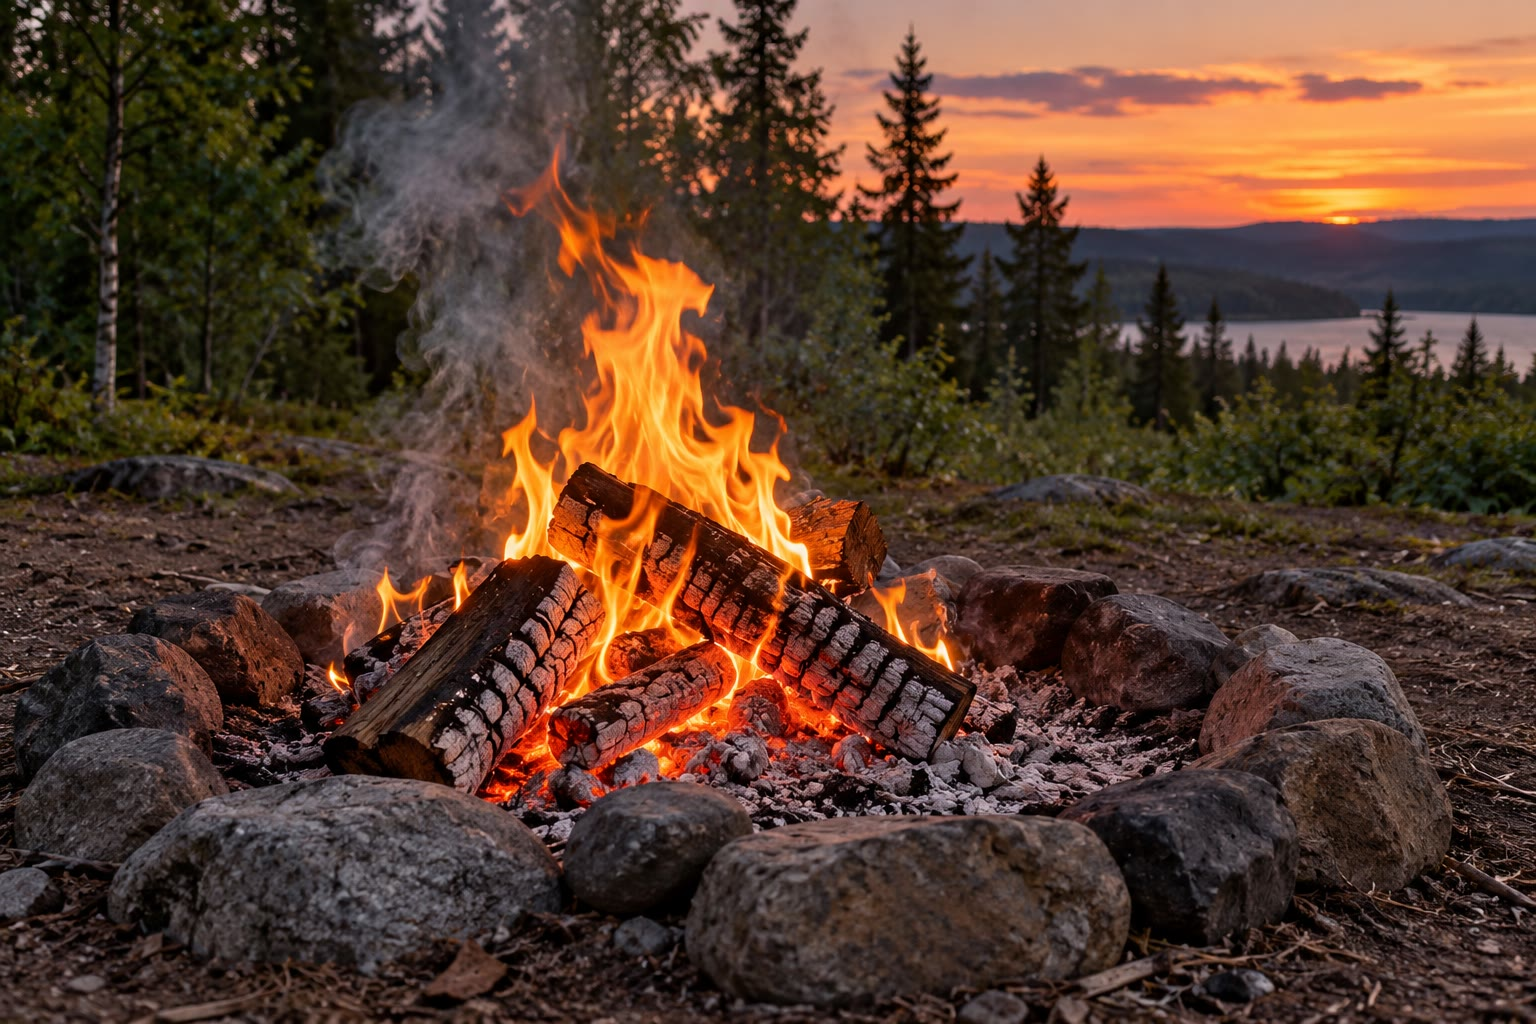
\includegraphics[width=0.6\linewidth]{images/book1/ai/g4-campfire.jpg}

{\small Uma fogueira: madeira, \omterm{def:g4:air-a-mixture-of-gases:air}{ar} e um fósforo --- e depois cinza e
fumaça.}
\end{omfigure}

\section{Os combustíveis}

\begin{definition}[Combustível]\label{def:g4:what-a-fire-needs:fuel}
Um \emph{combustível}\index{combustivel@combustível} é um material que pode queimar
e liberar calor e luz: a madeira, o papel, o carvão, a cera de vela, o
gás do fogão, a gasolina, o óleo de aquecimento.
\end{definition}

\begin{example}[Combustíveis sólidos, líquidos e gasosos]\label{ex:g4:what-a-fire-needs:fuels}
A madeira, o papel, o carvão e a cera de vela são \omterm{def:g4:what-a-fire-needs:fuel}{combustíveis} sólidos.
A gasolina e o óleo de aquecimento são \omterm{def:g4:what-a-fire-needs:fuel}{combustíveis} líquidos. O gás do
fogão da cozinha e o gás de um isqueiro são \omterm{def:g4:what-a-fire-needs:fuel}{combustíveis} gasosos.
\end{example}

\begin{remark}[Nem tudo queima]\label{rem:g4:what-a-fire-needs:not}
A pedra, a areia, o vidro e a água não queimam: eles não são
\omterm{def:g4:what-a-fire-needs:fuel}{combustíveis}. É por isso que uma lareira é construída de pedra ou de
tijolo, e que se usam areia e água para apagar incêndios.
\end{remark}

\section{O triângulo do fogo}

\begin{definition}[Triângulo do fogo]\label{def:g4:what-a-fire-needs:fire-triangle}
Um fogo precisa de três coisas ao mesmo tempo: um \omterm{def:g4:what-a-fire-needs:fuel}{combustível}, o
oxigênio do \omterm{def:g4:air-a-mixture-of-gases:air}{ar} e calor para começar. Essas três coisas são desenhadas
como os três lados de um triângulo, o \emph{triângulo do
fogo}\index{triangulo do fogo@triângulo do fogo}. Se falta um lado, não há fogo.
\end{definition}

\begin{omfigure}
\begin{tikzpicture}[font=\small]
  \coordinate (A) at (0,0); \coordinate (B) at (5,0); \coordinate (C) at (2.5,4.1);
  \draw[line width=3pt, brown!70!black] (A) -- (B);
  \draw[line width=3pt, omDef] (B) -- (C);
  \draw[line width=3pt, red!75!black] (C) -- (A);
  \node[below=4pt, font=\small\bfseries, brown!60!black] at (2.5,0) {combustível};
  \node[right=4pt, font=\small\bfseries, omDef] at (3.75,2.05) {oxigênio (do ar)};
  \node[left=4pt, font=\small\bfseries, red!75!black] at (1.25,2.05) {calor (para começar)};
  % a flame in the middle
  \fill[orange!80] (2.5,0.55) .. controls (1.95,1.15) and (2.35,1.75) .. (2.55,2.3)
    .. controls (2.75,1.75) and (3.05,1.15) .. (2.5,0.55);
  \fill[yellow!80] (2.5,0.7) .. controls (2.25,1.05) and (2.4,1.35) .. (2.52,1.65)
    .. controls (2.62,1.35) and (2.75,1.05) .. (2.5,0.7);
\end{tikzpicture}

{\small O \omterm{def:g4:what-a-fire-needs:fire-triangle}{triângulo do fogo}: \omterm{def:g4:what-a-fire-needs:fuel}{combustível}, oxigênio e calor, os três
juntos.}
\end{omfigure}

\begin{example}[Acender um fósforo]\label{ex:g4:what-a-fire-needs:match}
A cabeça de um fósforo é esfregada na lateral da caixinha. O atrito a
esquenta o bastante para ela começar a queimar: é o lado do calor no
triângulo. A madeira do fósforo é o \omterm{def:g4:what-a-fire-needs:fuel}{combustível}, e o \omterm{def:g4:air-a-mixture-of-gases:air}{ar} traz o
oxigênio.
\end{example}

\begin{example}[Soprar as brasas]\label{ex:g4:what-a-fire-needs:embers}
Brasas que parecem quase apagadas voltam a pegar fogo quando alguém
sopra nelas: o sopro traz mais \omterm{def:g4:air-a-mixture-of-gases:air}{ar}, e portanto mais oxigênio, para o
\omterm{def:g4:what-a-fire-needs:fuel}{combustível} que ainda está quente.
\end{example}

\section{Queimar fabrica substâncias novas}

\begin{definition}[Queima e combustão]\label{def:g4:what-a-fire-needs:burning}
A \emph{queima}\index{queima} é o que acontece quando um \omterm{def:g4:what-a-fire-needs:fuel}{combustível} tira
oxigênio do \omterm{def:g4:air-a-mixture-of-gases:air}{ar} e libera calor e luz. Os químicos chamam uma queima de
\emph{combustão}\index{combustao@combustão}. Durante uma combustão, o \omterm{def:g4:what-a-fire-needs:fuel}{combustível}
e o oxigênio são consumidos, e aparecem substâncias novas: fumaça,
cinza, dióxido de carbono e vapor de água.
\end{definition}

\begin{proposition}[Uma queima não pode ser desfeita]\label{prop:g4:what-a-fire-needs:new}
A cinza e a fumaça de um fogo não voltam a ser madeira, por mais que a
gente espere. Queimar fabrica substâncias novas que não estavam lá
antes; o \omterm{def:g4:what-a-fire-needs:fuel}{combustível} acabou para sempre.
\end{proposition}

\begin{inthelab}[Um copo frio sobre uma vela]
O professor segura por um instante um béquer de vidro frio e seco, de
boca para baixo, acima da chama de uma vela. O lado de dentro do vidro
fica embaçado com gotinhas minúsculas de água: o vapor de água fabricado
pela vela acesa voltou a ser líquido no vidro frio. Uma vela acesa
fabrica água, e também dióxido de carbono, que pode ser detectado com um
teste visto num capítulo mais adiante.
\end{inthelab}

\begin{omfigure}
\begin{tikzpicture}[font=\small, scale=1.3]
  % candle
  \fill[white, draw=black!50] (-0.25,0) rectangle (0.25,1.2);
  \draw[black!70] (0,1.2) -- (0,1.33);
  \fill[orange!85] (0,1.3) .. controls (-0.16,1.5) and (-0.06,1.75) .. (0,1.95)
    .. controls (0.06,1.75) and (0.16,1.5) .. (0,1.3);
  \fill[yellow!85] (0,1.36) .. controls (-0.08,1.5) and (-0.03,1.62) .. (0,1.72)
    .. controls (0.03,1.62) and (0.08,1.5) .. (0,1.36);
  % upturned cold beaker above
  \pic[transform shape, rotate=180] at (0,4.3) {beaker={0}{white}};
  \foreach \x/\y in {-0.6/3.9,-0.45/4.1,-0.2/3.95,0.1/4.15,0.35/3.9,0.6/4.05,
                     -0.7/3.5,0.7/3.4,-0.72/3.0,0.72/2.9}
    \fill[omDef!55] (\x,\y) circle (0.035);
  \draw[<-, omProp, thick] (0.68,3.95) -- (2.0,4.2) node[right, text=black]
    {gotinhas de água};
  \draw[<-, omProp, thick] (0.85,3.2) -- (2.0,3.3) node[right, text=black]
    {vidro frio, de boca para baixo};
  \draw[<-, omProp, thick] (0.15,1.7) -- (2.0,1.9) node[right, text=black]
    {a chama: a cera queimando};
  \draw[<-, omProp, thick] (0.3,0.6) -- (2.0,0.7) node[right, text=black]
    {a cera da vela: o combustível};
\end{tikzpicture}

{\small Um vidro frio segurado acima de uma vela fica embaçado: a cera
que \omterm{def:g4:what-a-fire-needs:burning}{queima} fabrica vapor de água.}
\end{omfigure}

\begin{example}[O que uma tora vira]\label{ex:g4:what-a-fire-needs:log}
Uma tora de alguns quilogramas \omterm{def:g4:what-a-fire-needs:burning}{queima} até virar um montinho de cinza. A
maior parte da madeira não sumiu: junto com o oxigênio do \omterm{def:g4:air-a-mixture-of-gases:air}{ar}, ela virou
fumaça, dióxido de carbono e vapor de água, que são gases e vão embora
para o céu.
\end{example}

\section{Apagar um fogo}

\begin{method}[Apagar um fogo: tirar um lado]\label{met:g4:what-a-fire-needs:out}
Para apagar um fogo, tire um lado do \omterm{def:g4:what-a-fire-needs:fire-triangle}{triângulo do fogo}:
\begin{itemize}
  \item \textbf{tire o oxigênio}: cubra o fogo com um cobertor
        antichamas, uma tampa ou areia, para que o \omterm{def:g4:air-a-mixture-of-gases:air}{ar} não chegue até
        ele;
  \item \textbf{tire o calor}: jogue água na madeira ou no papel que
        estão queimando, o que os esfria abaixo do ponto em que podem
        queimar;
  \item \textbf{tire o \omterm{def:g4:what-a-fire-needs:fuel}{combustível}}: feche o registro do gás, ou limpe a
        vegetação seca em volta de um incêndio florestal.
\end{itemize}
\end{method}

\begin{omfigure}
\begin{tikzpicture}[font=\small, scale=0.7]
  \foreach \k/\lab/\side in {0/{um cobertor: sem oxigênio}/1, 1/{água: sem calor}/2,
                              2/{gás fechado: sem combustível}/0} {
    \begin{scope}[xshift=\k*6.2cm]
      \coordinate (A) at (0,0); \coordinate (B) at (4,0); \coordinate (C) at (2,3.3);
      \pgfmathsetmacro\oa{\side==0 ? 0.2 : 1}
      \pgfmathsetmacro\ob{\side==1 ? 0.2 : 1}
      \pgfmathsetmacro\oc{\side==2 ? 0.2 : 1}
      \draw[line width=2.5pt, brown!70!black, opacity=\oa] (A) -- (B);
      \draw[line width=2.5pt, omDef, opacity=\ob] (B) -- (C);
      \draw[line width=2.5pt, red!75!black, opacity=\oc] (C) -- (A);
      \ifnum\side=0 \draw[line width=1.4pt, black] (1.6,-0.4) -- (2.4,0.4) (1.6,0.4) -- (2.4,-0.4);\fi
      \ifnum\side=1 \draw[line width=1.4pt, black] (2.6,1.25) -- (3.4,2.05) (2.6,2.05) -- (3.4,1.25);\fi
      \ifnum\side=2 \draw[line width=1.4pt, black] (0.6,1.25) -- (1.4,2.05) (0.6,2.05) -- (1.4,1.25);\fi
      \node[align=center, anchor=north] at (2,-0.6) {\lab};
    \end{scope}
  }
\end{tikzpicture}

{\small Três jeitos de apagar um fogo, cada um tirando um lado do
triângulo (riscado): o oxigênio, o calor ou o \omterm{def:g4:what-a-fire-needs:fuel}{combustível}.}
\end{omfigure}

\begin{omfigure}
\begin{minipage}[t]{0.48\linewidth}\centering
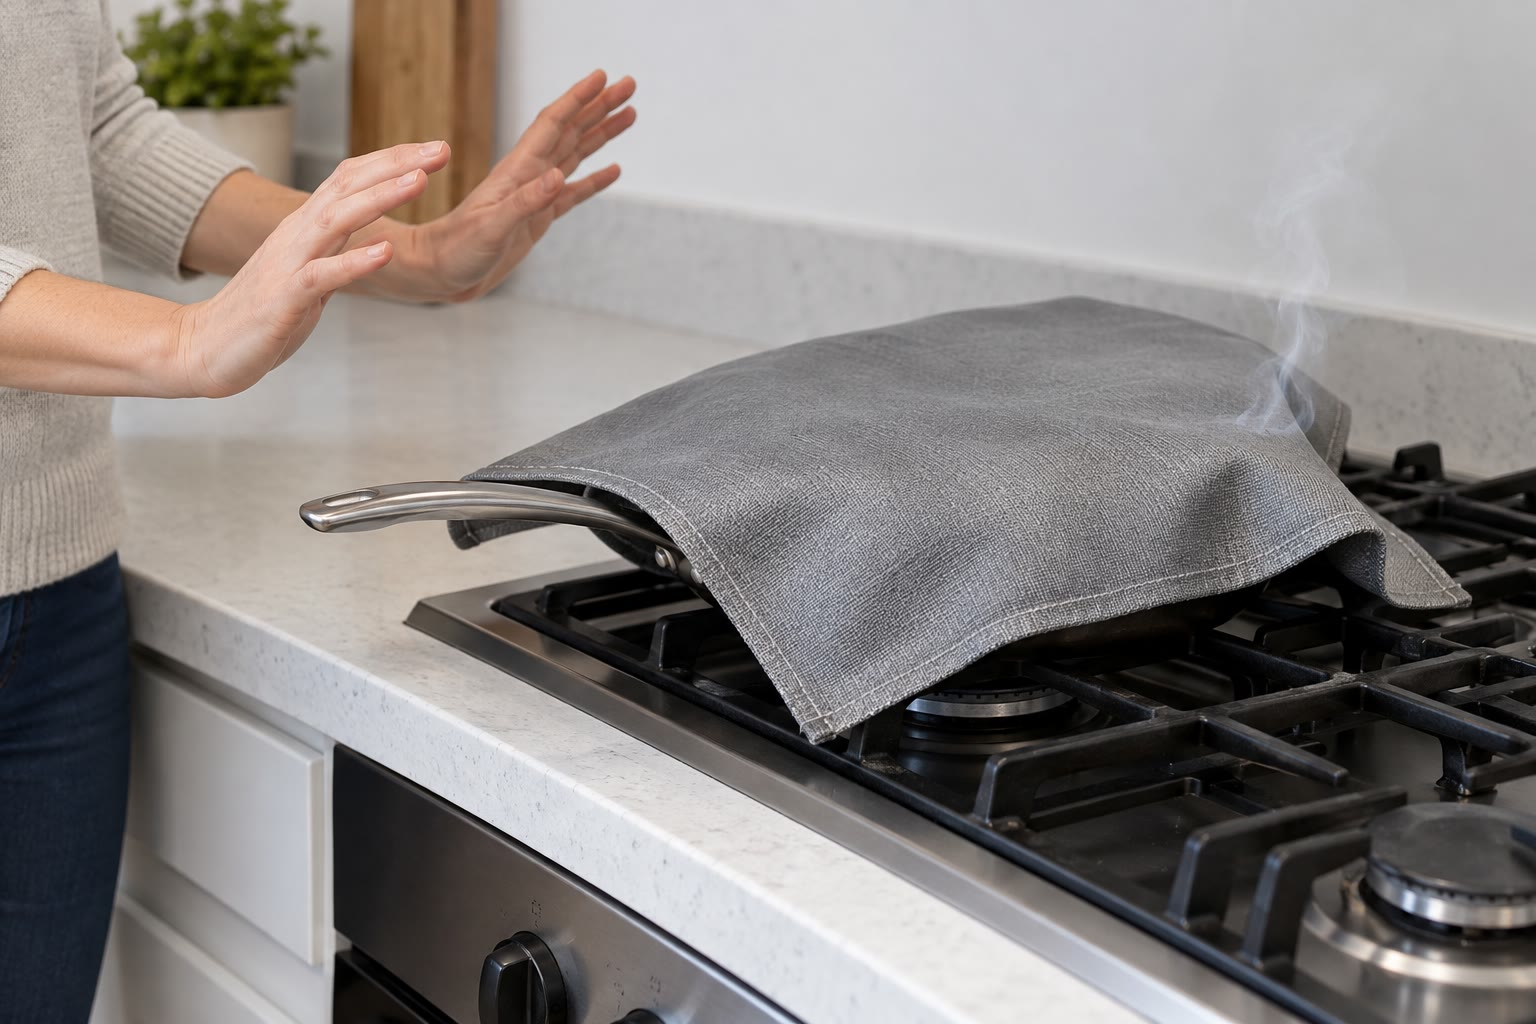
\includegraphics[width=\linewidth,height=4.6cm,keepaspectratio]{images/book1/ai/g4-fire-blanket.jpg}

{\small Um cobertor antichamas sobre uma panela: o \omterm{def:g4:air-a-mixture-of-gases:air}{ar} não chega mais ao
fogo.}
\end{minipage}\hfill
\begin{minipage}[t]{0.48\linewidth}\centering
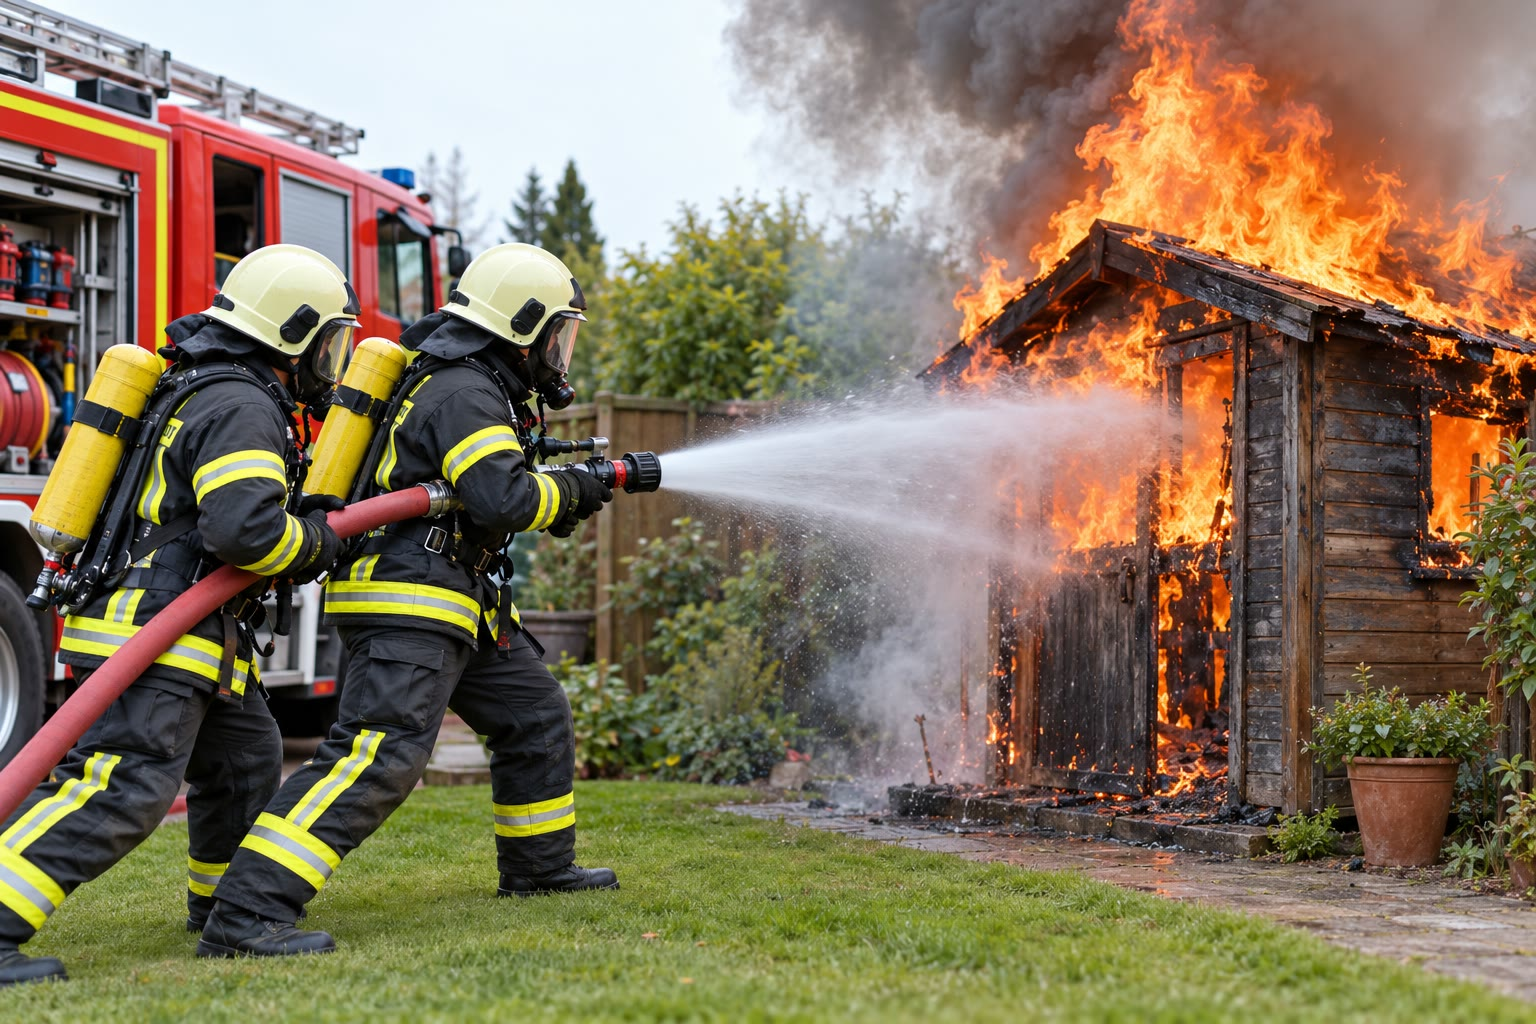
\includegraphics[width=\linewidth,height=4.6cm,keepaspectratio]{images/book1/ai/g4-firefighters.jpg}

{\small Bombeiros jogam água para esfriar um galpão em chamas.}
\end{minipage}
\end{omfigure}

\section{Segurança contra incêndios}

\begin{remark}[Nunca jogue água numa panela de óleo em chamas]\label{rem:g4:what-a-fire-needs:oil}
Se o óleo de uma frigideira pegar fogo, ninguém deve jogar água nele: a
água ferve na hora debaixo do óleo e espirra óleo em chamas para fora
da panela. Um adulto desliga o gás ou a chapa elétrica e cobre a panela
com uma tampa ou com um cobertor antichamas.
\end{remark}

\begin{safety}{\ghs{GHS02}\ghs{GHS04}}
% ledger: ghs:butane
O gás de um isqueiro ou de um cartucho de camping é o butano. O
pictograma da chama (GHS02) quer dizer: extremamente inflamável, manter
longe de chamas e faíscas. O pictograma do cilindro de gás (GHS04) quer
dizer: um gás guardado sob pressão.
\end{safety}

\begin{proposition}[O que fazer num incêndio]\label{prop:g4:what-a-fire-needs:safety}
A fumaça é o primeiro perigo de um incêndio: ela é quente, esconde a
saída e é venenosa para respirar. Um detector de fumaça no teto apita
alto assim que a fumaça chega até ele. Se houver um incêndio: saia,
fique abaixado, por baixo da fumaça, feche as portas depois de passar e
chame os bombeiros lá de fora. Nunca volte para dentro.
\end{proposition}

\begin{omfigure}
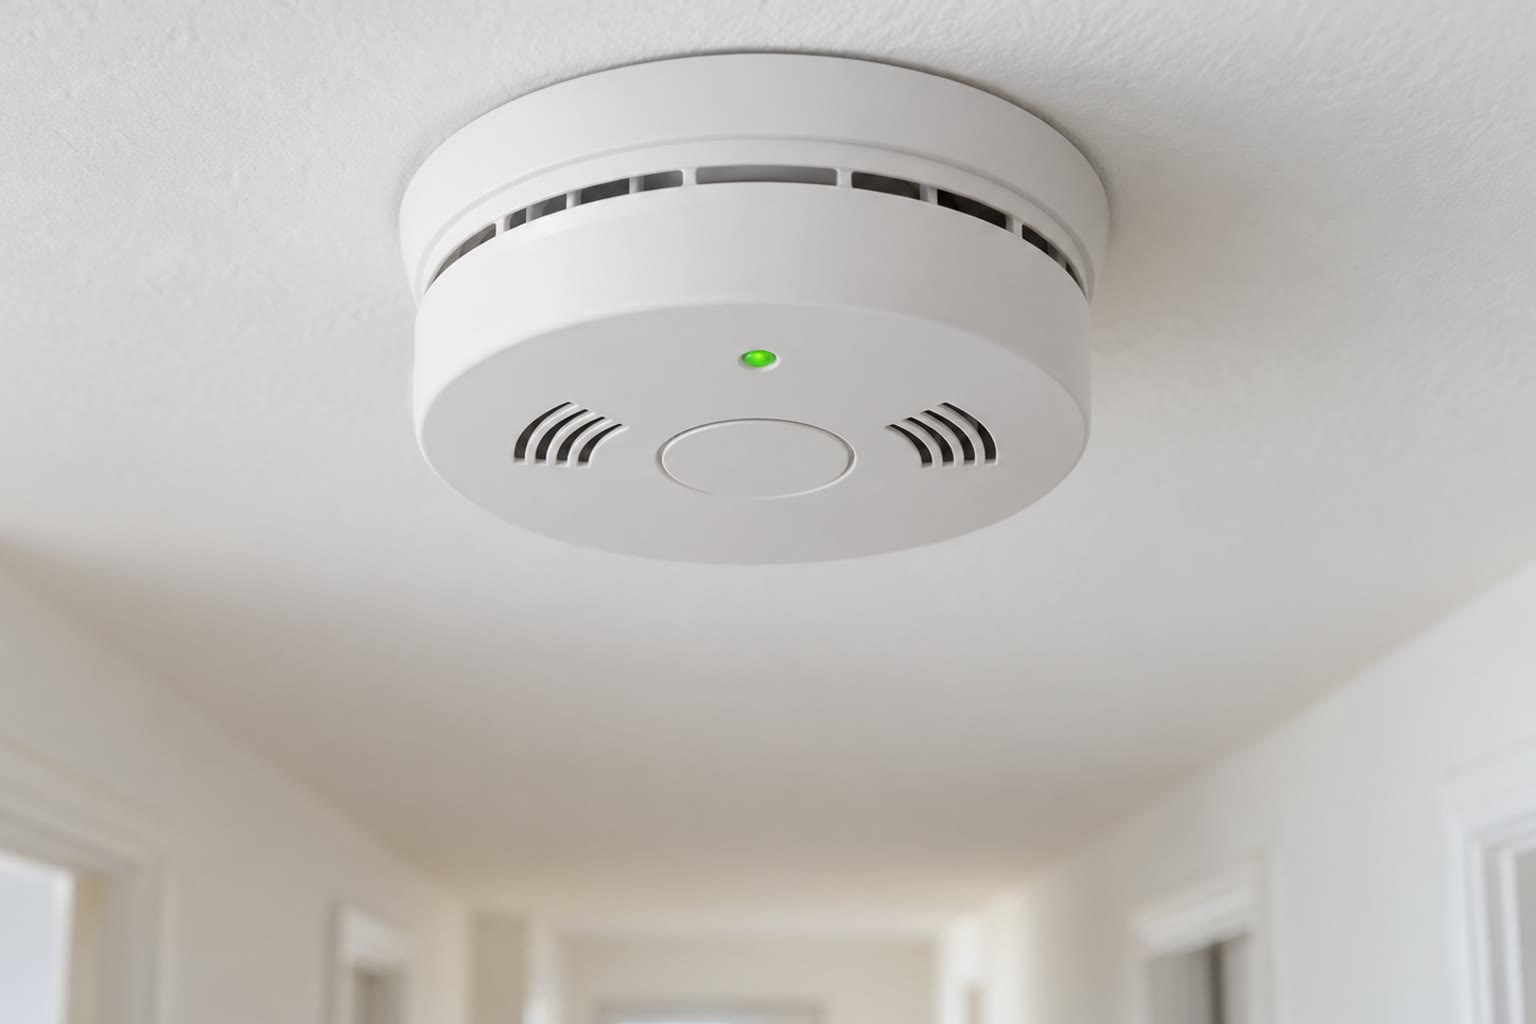
\includegraphics[width=0.42\linewidth]{images/book1/ai/g4-smoke-alarm.jpg}

{\small Um detector de fumaça: ele dispara assim que a fumaça chega até
ele.}
\end{omfigure}

\section{Exercícios}

\begin{exercise}[$\star$]\label{exo:g4:what-a-fire-needs:1}
Diga os três lados do \omterm{def:g4:what-a-fire-needs:fire-triangle}{triângulo do fogo}.
\end{exercise}

\begin{exercise}[$\star$]\label{exo:g4:what-a-fire-needs:2}
Quais destes são \omterm{def:g4:what-a-fire-needs:fuel}{combustíveis}: madeira, areia, cera de vela, vidro,
gasolina, água, papel?
\end{exercise}

\begin{exercise}[$\star$]\label{exo:g4:what-a-fire-needs:3}
Um cobertor antichamas é jogado sobre um pequeno fogo. Que lado do
\omterm{def:g4:what-a-fire-needs:fire-triangle}{triângulo do fogo} ele tira?
\end{exercise}

\begin{exercise}[$\star$]\label{exo:g4:what-a-fire-needs:4}
Bombeiros jogam água num galpão em chamas. Que lado do \omterm{def:g4:what-a-fire-needs:fire-triangle}{triângulo do fogo}
a água tira?
\end{exercise}

\begin{exercise}[$\star$]\label{exo:g4:what-a-fire-needs:5}
Diga três substâncias novas fabricadas quando a madeira \omterm{def:g4:what-a-fire-needs:burning}{queima}.
\end{exercise}

\begin{exercise}[$\star$]\label{exo:g4:what-a-fire-needs:6}
Por que soprar as brasas faz o fogo pegar de novo?
\end{exercise}

\begin{exercise}[$\star$]\label{exo:g4:what-a-fire-needs:7}
Um copo frio segurado acima de uma vela fica embaçado. Que substância
nova a vela fabricou?
\end{exercise}

\begin{exercise}[$\star$]\label{exo:g4:what-a-fire-needs:8}
O que você deve fazer primeiro se um detector de fumaça disparar e você
vir fumaça?
\end{exercise}

\begin{exercise}[$\star$]\label{exo:g4:what-a-fire-needs:9}
Olhe a figura dos três triângulos pequenos. Que lado está riscado quando
o gás é fechado?
\end{exercise}

\begin{exercise}[$\star\star$]\label{exo:g4:what-a-fire-needs:10}
Para deter um incêndio florestal, os bombeiros às vezes cortam uma faixa
larga de árvores na frente dele. Que lado do \omterm{def:g4:what-a-fire-needs:fire-triangle}{triângulo do fogo} eles
estão tirando?
\end{exercise}

\begin{exercise}[$\star\star$]\label{exo:g4:what-a-fire-needs:11}
Uma tora pesa muito mais do que a cinza dela. Uma parte da tora
desapareceu? Explique para onde ela foi.
\end{exercise}
